%------------------------------------------------
\begin{frame}
 \frametitle{Fast switches\footnote{developed together with Fa.\ barthel HF-Technik GmbH, Aachen} for RF power of Wien filter}
 
\vspace{-0.2cm} 
\begin{columns}
 \column{0.52\textwidth}
\begin{small}
\textbf{GaN HEMT-based solution (Gallium Nitride Transistors):}
 \begin{itemize}
    \item Short switch on/off times ($\approx$ few ns).
    \item High power capabilities ($\approx$ few kV).
    \item On board power damping.
  \end{itemize}
\end{small}
 
 \column{0.5\textwidth}
 \begin{center}
  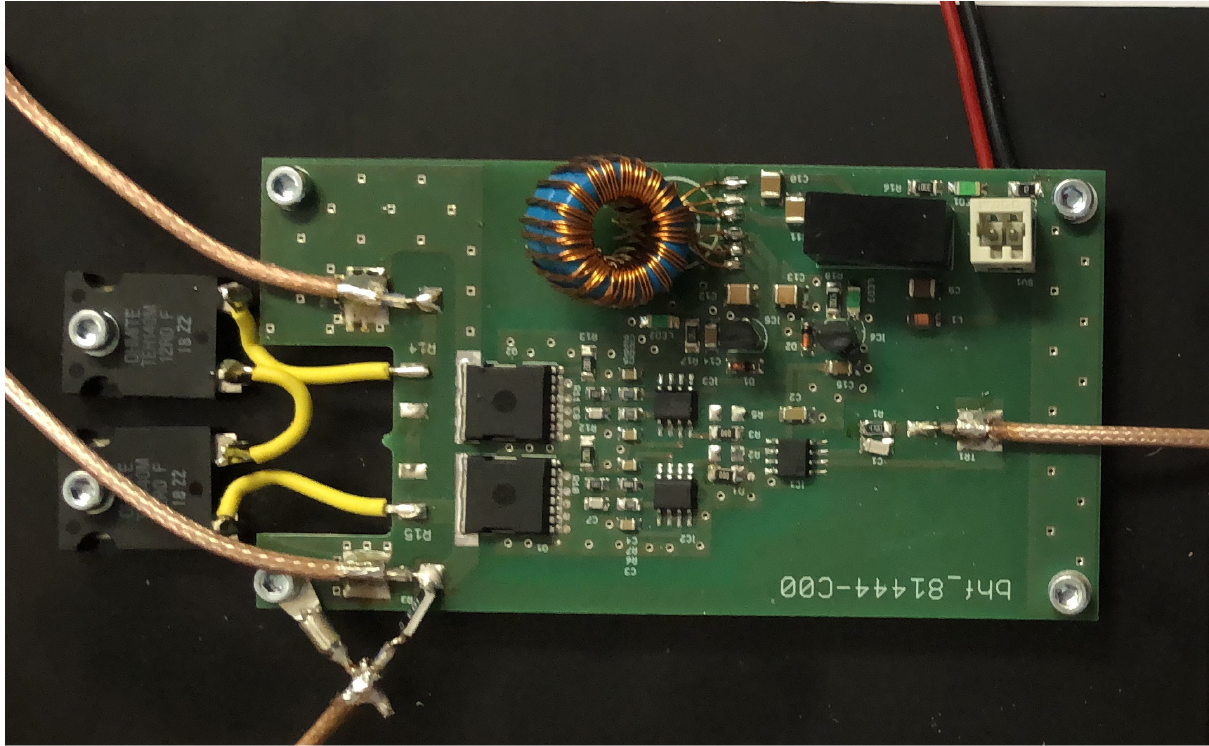
\includegraphics[width = 0.75\textwidth]{fast-switch}
 \end{center}
\end{columns}
 
\vspace{-0.4cm} 
\begin{columns}
 \column{0.46\textwidth}
  \begin{center}
  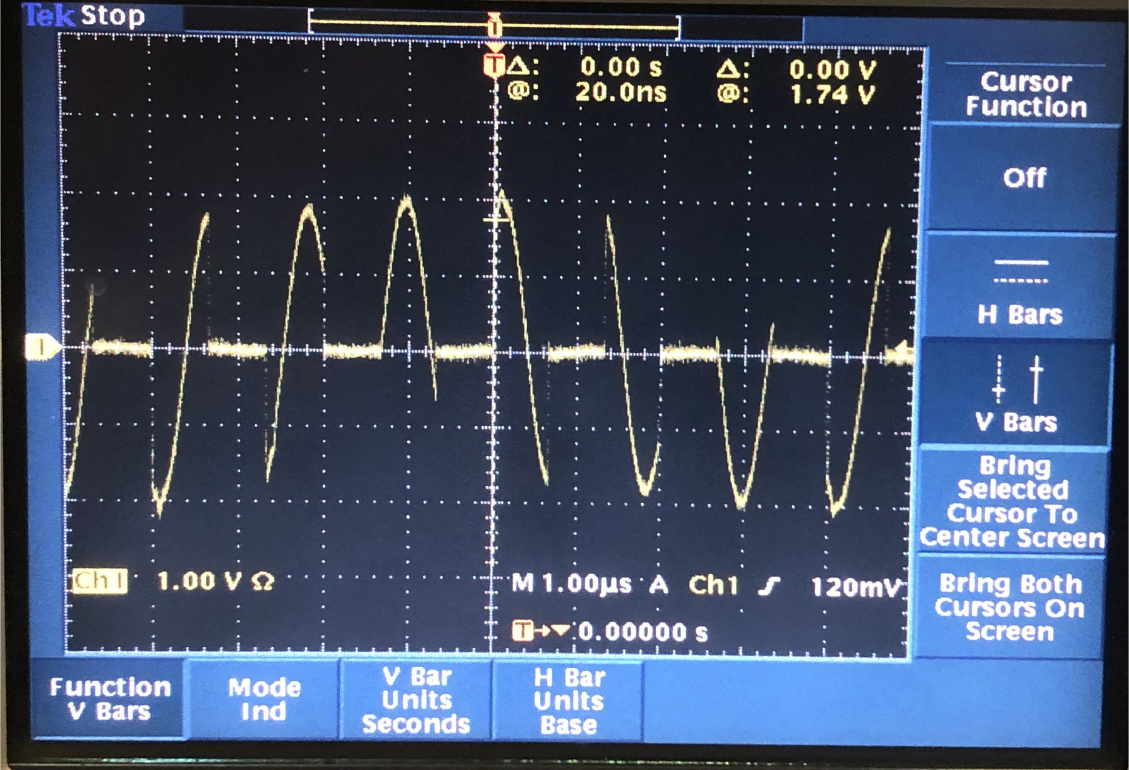
\includegraphics[width = 0.75\textwidth]{osci-fast-switch}
 \end{center}
 
 \column{0.54\textwidth}
\begin{small}
 \begin{itemize}
 \item symmetric switch on/off times ($\approx$ few ns).
 \item $-\SI{30}{\decibel}$ power damping.
  \end{itemize}
\end{small}
\end{columns}

\vspace{-0.2cm}  
\begin{alertblock}{Installed switches:}
\begin{itemize}
 \item capable to handle up to \SI{200}{W} each
 \item permits system to run near a total power of \SI{0.8}{kW} in pulsed mode
\end{itemize}
\end{alertblock}
  

\end{frame}
%------------------------------------------------
